\begin{figure}[h]
	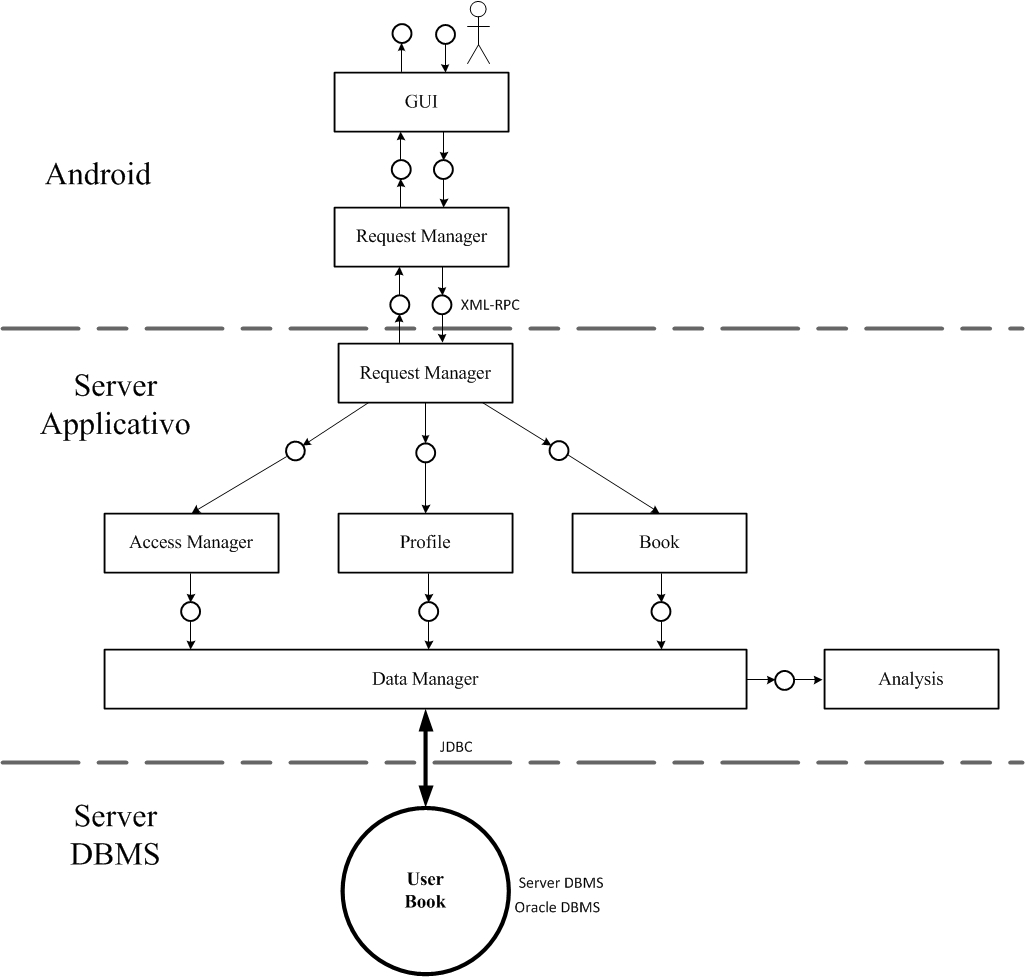
\includegraphics[width=0.8\textwidth]{Immagini/Architettura_Software}
	\caption{Architettura Software}
	\label{fig:ArchitetturaSoftware}
\end{figure}
\newpage
Nella figura ~\ref{fig:ArchitetturaSoftware} è mostrata l'architettura software modellizzata attraverso una rete di Petri. Innanzitutto si può già osservare chè è stata definita seguendo il modello architetturale MVC:
\begin{itemize}
	\item A monte è prevista una parte riservata all'interfaccia grafica, attraverso la quale sarà possibile inviare e ricevere informazioni dal server applicativo. Si vede, infatti, che è prevista una comunicazione bidirezionale tra dispositivo Android e Server.
	\item Al centro sono rappresentate tutte le richieste a cui è in grado di rispondere. Queste, quindi, saranno funzioni implementate lato Server.
	\item Infine, è prevista una banca dati persistente, in questo caso un database relazione, al quale il Server Applicativo accede sia per operazioni di lettura che di scrittura, sempre con lo scopo di far fronte alle richieste provenienti a monte.
\end{itemize}
Si può quindi constatare che non si trattano di strati tra loro indipendenti, poichè il flusso dei dati li coinvolge tutti.